\documentclass[fleqn]{article}
\usepackage[spanish]{babel}
\usepackage{amsmath, amssymb, amsfonts}
\usepackage{parskip}
\usepackage{enumerate}
\usepackage{nopageno}
\usepackage[left = 24mm, right = 24mm, bottom = 21mm, top = 21mm]{geometry}
\usepackage{graphicx}
\usepackage{wrapfig}

\usepackage{heuristica}
\usepackage[heuristica,vvarbb,bigdelims]{newtxmath}
\usepackage[T1]{fontenc}
\renewcommand*\oldstylenums[1]{\textosf{#1}}

\begin{document}
    4. Demuestra o da un contraejemplo. Para $ i = 1,2,3 $, sea $ G_i $ una gráfica.
    \begin{enumerate}[a)]
        \item $ G_1 + G_2 = G_2 + G_1 $
        
        \textbf{Demostración.}

        Ya que 
        \begin{align*}
            V \left( G_1 + G_2 \right) &= V \left( G_1 \right) \cup V \left( G_2 \right) \\
            &= V \left( G_2 \right) \cup V \left( G_1 \right) \\
            &= V \left( G_2 + G_1 \right)
        \end{align*}
        y
        \begin{align*}
            A \left( G_1 + G_2 \right) &= A \left( G_1 \right) \cup A \left( G_2 \right) \cup \left\lbrace uv \mid u \in V \left( G_1 \right), v \in V \left( G_2 \right) \right\rbrace \\
            &= A \left( G_2 \right) \cup A \left( G_1 \right) \cup \left\lbrace vu \mid v \in V \left( G_2 \right), u \in V \left( G_1 \right) \right\rbrace \\
            &= A \left( G_2 + G_1 \right) 
        \end{align*}
        se tiene que $ G_1 + G_2 = G_2 + G_1 $ \hfill $ \blacksquare $

        \item $ G_1 \times G_2 = G_2 \times G_1 $
        
        \textbf{Afirmación:} $ G_1 \times G_2 \neq G_2 \times G_1 $

        Sean $ G_1 = \left( V, A \right) $ y $ G_2 = \left( V, A \right) $ gráficas con $ V \left( G_1 \right) = \left\lbrace u_1, u_2 \right\rbrace $, $ A \left( G_1 \right) = \left\lbrace u_1u_2 \right\rbrace $, $ V \left( G_2 \right) = \left\lbrace v_1, v_2, v_3 \right\rbrace $ y $ A \left( G_2 \right) = \left\lbrace v_1v_2, v_2v_3 \right\rbrace $.

        \begin{minipage}{0.75\textwidth}
            Como
            \begin{align*}
                V \left( G_1 \times G_2 \right) &= V \left( G_1 \right) \times V \left( G_2 \right) \\
                & = \left\lbrace \left( u_1, v_1 \right), \left( u_1, v_2 \right), \left( u_1, v_3 \right), \left( u_2, v_1 \right), \left( u_2, v_2 \right), \left( u_2, v_3 \right) \right\rbrace \\
                & \neq \left\lbrace \left( v_1, u_1 \right), \left( v_1, u_2 \right), \left( v_2, u_1 \right), \left( v_2, u_2 \right), \left( v_3, u_1 \right), \left( v_3, u_2 \right) \right\rbrace \\
                & = V \left( G_2 \right) \times V \left( G_1 \right) \\
                & = V \left( G_2 \times G_1 \right)
            \end{align*} 
            se tiene que $ G_1 \times G_2 \neq G_2 \times G_1 $
        \end{minipage}
        \begin{minipage}{0.25\textwidth}
            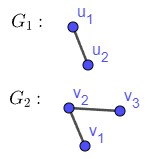
\includegraphics[scale = 0.9]{G1 y G2.jpg}
        \end{minipage}

        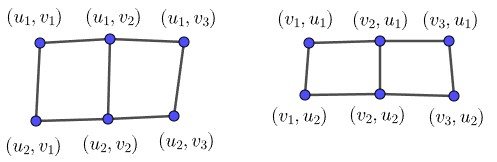
\includegraphics[scale = 0.9]{G1xG2.jpg}

        \item $ \left( G_1 + G_2 \right) + G_3 = G_1 + \left( G_2 + G_3 \right) $
        
        \textbf{Demostración.}
        \begin{align*}
            V \left( \left( G_1 + G_2 \right) + G_3 \right) &= V \left( G_1 + G_2 \right) \cup V \left( G_3 \right) \\
            &= \left[ V \left( G_1 \right) \cup V \left( G_2 \right) \right] \cup V \left( G_3 \right) \\
            &= V \left( G_1 \right) \cup \left[ V \left( G_2 \right) \cup V \left( G_3 \right) \right] \\
            &= V \left( G_1 \right) \cup V \left( G_2 + G_3 \right) \\
            &= V \left( G_1 + \left( G_2 + G_3 \right) \right)
        \end{align*}
        Ahora, sea $ uv \in A \left( \left( G_1 + G_2 \right) + G_3 \right) $. P.d. $ uv \in A \left( G_1 + \left( G_2 + G_3 \right) \right) $.

        Ya que 
        \begin{align*}
            A \left( \left( G_1 + G_2 \right) + G_3 \right) &= A \left( G_1 + G_2 \right) \cup A \left( G_3 \right) \cup \left\lbrace ab \mid a \in V \left( G_1 + G_2 \right), b \in V \left( G_3 \right) \right\rbrace \\
            &= A \left( G_1 \right) \cup A \left( G_2 \right) \cup \left\lbrace ab \mid a \in V \left( G_1 \right), b \in V \left( G_2 \right) \right\rbrace \cup A \left( G_3 \right) \cup \\
            & \hspace{4mm} \left\lbrace ab \mid a \in V \left( G_1 + G_2 \right), b \in V \left( G_3 \right) \right\rbrace
        \end{align*}
        se dan los siguientes casos:

        \begin{itemize}
            \item Si $ uv \in A \left( G_1 \right) $ entonces $ uv \in A \left( G_1 \right) \cup A \left( G_2 + G_3 \right) \cup \left\lbrace ab \mid a \in V \left( G_1 \right), b \in V \left( G_2 + G_3 \right) \right\rbrace $, es decir, \\ $ uv \in A \left( G_1 + \left( G_2 + G_3 \right) \right) $.
            
            \item Si $ uv \in A \left( G_2 \right) $ entonces $ uv \in A \left( G_1 \right) \cup A \left( G_2 \right) \cup A \left( G_3 \right) \cup \left\lbrace ab \mid a \in V \left( G_2 \right), b \in V \left( G_3 \right) \right\rbrace \cup $ \\ $ \left\lbrace ab \mid a \in V \left( G_1 \right), b \in V \left( G_2 + G_3 \right) \right\rbrace $, es decir, $ uv \in A \left( G_1 + \left( G_2 + G_3 \right) \right) $.
            
            \item Si $ uv \in A \left( G_3 \right) $ entonces $ uv \in A \left( G_1 \right) \cup A \left( G_2 \right) \cup A \left( G_3 \right) \cup \left\lbrace ab \mid a \in V \left( G_2 \right), b \in V \left( G_3 \right) \right\rbrace \cup $ \\ $ \left\lbrace ab \mid a \in V \left( G_1 \right), b \in V \left( G_2 + G_3 \right) \right\rbrace $, es decir, $ uv \in A \left( G_1 + \left( G_2 + G_3 \right) \right) $.
            
            \item Si $ uv \in \left\lbrace ab \mid a \in V \left( G_1 \right), b \in V \left( G_2 \right) \right\rbrace $ entonces $ uv \in \left\lbrace ab \mid a \in V \left( G_1 \right), b \in V \left( G_2 \right) \cup V \left( G_3 \right) \right\rbrace = $ \\ $ \left\lbrace ab \mid a \in V \left( G_1 \right), b \in V \left( G_2 + G_3 \right) \right\rbrace $, es decir, $ uv \in A \left( G_1 + \left( G_2 + G_3 \right) \right) $.
            
            \item Si $ uv \in \left\lbrace ab \mid a \in V \left( G_1 + G_2 \right), b \in V \left( G_3 \right) \right\rbrace = \left\lbrace ab \mid a \in V \left( G_1 \right) \cup V \left( G_2 \right), b \in V \left( G_3 \right) \right\rbrace $ entonces se tienen los siguientes casos:
            
            \begin{itemize}
                \item Si $ u \in V \left( G_1 \right) $ entonces $ uv \in \left\lbrace ab \mid a \in V \left( G_1 \right), b \in V \left( G_3 \right) \right\rbrace $. Así, \\ $ uv \in \left\lbrace ab \mid a \in V \left( G_1 \right), b \in V \left( G_2 \right) \cup V \left( G_3 \right) \right\rbrace = \left\lbrace ab \mid a \in V \left( G_1 \right), b \in V \left( G_2 + G_3 \right)\right\rbrace $. De esta manera, $ uv \in A \left( G_1 \right) \cup A \left( G_2 + G_3 \right) \cup \left\lbrace ab \mid a \in V \left( G_1 \right), b \in V \left( G_2 + G_3 \right)\right\rbrace $, es decir, \\ $ uv \in A \left( G_1 + \left( G_2 + G_3 \right) \right) $.
                
                \item Si $ u \in V \left( G_2 \right) $ entonces $ uv \in \left\lbrace ab \mid a \in V \left( G_2 \right), b \in V \left( G_3 \right) \right\rbrace $. De esta forma, $ uv \in A \left( G_1 \right) \cup A \left( G_2 \right) \cup A \left( G_3 \right) \cup \left\lbrace ab \mid a \in V \left( G_2 \right), b \in V \left( G_3 \right) \right\rbrace \cup \left\lbrace ab \mid a \in V \left( G_1 \right), b \in V \left( G_2 + G_3 \right) \right\rbrace $, es decir, \\ $ uv \in A \left( G_1 + \left( G_2 + G_3 \right) \right) $.
            \end{itemize}
        \end{itemize}

        Por lo anterior, $ A \left( \left( G_1 + G_2 \right) + G_3 \right) \subseteq A \left( G_1 + \left( G_2 + G_3 \right) \right) $.

        Por otro lado, sea $ uv \in A \left( G_1 + \left( G_2 + G_3 \right) \right) $. P.d. $ uv \in A \left( \left( G_1 + G_2 \right) + G_3 \right) $.
        
        Como
        \begin{align*}
            A \left( G_1 + \left( G_2 + G_3 \right) \right) &= A \left( G_1 \right) \cup A \left( G_2 + G_3 \right) \cup \left\lbrace ab \mid a \in V \left( G_1 \right), b \in V \left( G_2 + G_3 \right) \right\rbrace \\
            &= A \left( G_1 \right) \cup A \left( G_2 \right) \cup A \left( G_3 \right) \cup \left\lbrace ab \mid a \in V \left( G_2 \right), b \in V \left( G_3 \right) \right\rbrace \cup \\
            & \hspace{4mm} \left\lbrace ab \mid a \in V \left( G_1 \right), b \in V \left( G_2 + G_3 \right) \right\rbrace
        \end{align*}
        se dan los siguientes casos:

        \begin{itemize}
            \item Si $ uv \in A \left( G_1 \right) $ entonces $ uv \in A \left( G_1 \right) \cup A \left( G_2 \right) \cup \left\lbrace ab \mid a \in V \left( G_1 \right), b \in V \left( G_2 \right) \right\rbrace \cup A \left( G_3 \right) \cup $ \\ $ \left\lbrace ab \mid a \in V \left( G_1 + G_2 \right), b \in V \left( G_3 \right) \right\rbrace $, es decir, $ uv \in A \left( \left( G_1 + G_2 \right) + G_3 \right) $.
            
            \item Si $ uv \in A \left( G_2 \right) $ entonces $ uv \in A \left( G_1 \right) \cup A \left( G_2 \right) \cup \left\lbrace ab \mid a \in V \left( G_1 \right), b \in V \left( G_2 \right) \right\rbrace \cup A \left( G_3 \right) \cup $ \\ $ \left\lbrace ab \mid a \in V \left( G_1 + G_2 \right), b \in V \left( G_3 \right) \right\rbrace $, es decir, $ uv \in A \left( \left( G_1 + G_2 \right) + G_3 \right) $.
            
            \item Si $ uv \in A \left( G_3 \right) $ entonces $ uv \in A \left( G_1 + G_2 \right) \cup A \left( G_3 \right) \cup \left\lbrace ab \mid a \in V \left( G_1 + G_2 \right), b \in V \left( G_3 \right) \right\rbrace $, es decir, \\ $ uv \in A \left( \left( G_1 + G_2 \right) + G_3 \right) $.
            
            \item Si $ uv \in \left\lbrace ab \mid a \in V \left( G_2 \right), b \in V \left( G_3 \right) \right\rbrace $ entonces $ uv \in \left\lbrace ab \mid a \in V \left( G_1 \right) \cup V \left( G_2 \right), b \in V \left( G_3 \right) \right\rbrace = $ \\ $ \left\lbrace ab \mid a \in V \left( G_1 + G_2 \right), b \in V \left( G_3 \right) \right\rbrace $. Así, $ uv \in A \left( G_1 + G_2 \right) \cup A \left( G_3 \right) \cup \left\lbrace ab \mid a \in V \left( G_1 + G_2 \right), b \in V \left( G_3 \right) \right\rbrace $, es decir, $ uv \in A \left( \left( G_1 + G_2 \right) + G_3 \right) $.
            
            \item Si $ uv \in \left\lbrace ab \mid a \in V \left( G_1 \right), b \in V \left( G_2 + G_3 \right) \right\rbrace = \left\lbrace ab \mid a \in V \left( G_1 \right), b \in V \left( G_2 \right) \cup V \left( G_3 \right) \right\rbrace $ entonces se tienen los siguientes casos:
            
            \begin{itemize}
                \item Si $ v \in V \left( G_2 \right) $ entonces $ uv \in \left\lbrace ab \mid a \in V \left( G_1 \right), b \in V \left( G_2 \right) \right\rbrace $. Así, $ uv \in A \left( G_1 \right) \cup A \left( G_2 \right) \cup $ \\ $ \left\lbrace ab \mid a \in V \left( G_1 \right), b \in V \left( G_2 \right) \right\rbrace \cup A \left( G_3 \right) \cup \left\lbrace ab \mid a \in V \left( G_1 + G_2 \right), b \in V \left( G_3 \right) \right\rbrace $. De esta manera, \\ $ uv \in A \left( \left( G_1 + G_2 \right) + G_3 \right) $.
                
                \item Si $ v \in V \left( G_3 \right) $ entonces $ uv \in \left\lbrace ab \mid a \in V \left( G_1 \right), b \in V \left( G_3 \right) \right\rbrace \subseteq \left\lbrace ab \mid a \in V \left( G_1 \right) \cup V \left( G_2 \right), b \in V \left( G_3 \right) \right\rbrace $. Así, $ uv \in \left\lbrace ab \mid a \in V \left( G_1 + G_2 \right), b \in V \left( G_3 \right) \right\rbrace $. De esta manera, $ uv \in A \left( G_1 + G_2 \right) \cup A \left( G_3 \right) \cup $ \\ $ \left\lbrace ab \mid a \in V \left( G_1 + G_2 \right), b \in V \left( G_3 \right) \right\rbrace $, es decir, $ uv \in A \left( \left( G_1 + G_2 \right) + G_3 \right) $.
            \end{itemize}
        \end{itemize}

        Por lo anterior, $ A \left( \left( G_1 + G_2 \right) + G_3 \right) \supseteq A \left( G_1 + \left( G_2 + G_3 \right) \right) $.

        Por lo tanto, $ A \left( \left( G_1 + G_2 \right) + G_3 \right) = A \left( G_1 + \left( G_2 + G_3 \right) \right) $. En conclusión, $ \left( G_1 + G_2 \right) + G_3 = G_1 + \left( G_2 + G_3 \right) $.
        
        \item $ \left( G_1 \times G_2 \right) \times G_3 = G_1 \times \left( G_2 \times G_3 \right) $
        
        \textbf{Afirmación:} $ \left( G_1 \times G_2 \right) \times G_3 \neq G_1 \times \left( G_2 \times G_3 \right) $.

        Sean $ G_1 = \left( V, A \right) $, $ G_2 = \left( V, A \right) $ y $ G_3 = \left( V, A \right) $ gráficas con $ V \left( G_1 \right) = \left\lbrace u_1 \right\rbrace $, $ A \left( G_1 \right) = \emptyset $, $ V \left( G_2 \right) = \left\lbrace v_1, v_2 \right\rbrace $, $ A \left( G_2 \right) = \left\lbrace v_1v_2 \right\rbrace $, $ V \left( G_3 \right) = \left\lbrace w_1, w_2, w_3 \right\rbrace $ y $ A \left( G_3 \right) = \left\lbrace w_1w_2, w_2w_3 \right\rbrace $. 

        Como
        \begin{align*}
            V \left( \left( G_1 \times G_2 \right) \times G_3 \right) &= V \left( G_1 \times G_2 \right) \times V \left( G_3 \right) \\
            & = \left[ V \left( G_1 \right) \times V \left( G_2 \right) \right] \times V \left( G_3 \right) \\
            & = \left\lbrace \left( \left( u_1, v_1 \right), w_1 \right), \left( \left( u_1, v_1 \right), w_2 \right), \left( \left( u_1, v_1 \right), w_3 \right), \left( \left( u_1, v_2 \right), w_1 \right), \left( \left( u_1, v_2 \right), w_2 \right), \right. \\
            & \hspace{4mm} \left. \left( \left( u_1, v_2 \right), w_3 \right) \right\rbrace \\
            & \neq \left\lbrace \left( u_1, \left( v_1, w_1 \right) \right), \left( u_1, \left( v_1, w_2 \right) \right), \left( u_1, \left( v_1, w_3 \right) \right), \left( u_1, \left( v_2, w_1 \right) \right), \left( u_1, \left( v_2, w_2 \right) \right), \right. \\
            & \hspace{4mm} \left. \left( u_1, \left( v_2, w_3 \right) \right) \right\rbrace \\
            & = V \left( G_1 \right) \times \left[ V \left( G_2 \right) \times V \left( G_3 \right) \right]\\
            & = V \left( G_1 \right) \times V \left( G_2 \times G_3 \right) \\
            & = V \left( G_1 \times \left( G_2 \times G_3 \right) \right)
        \end{align*} 
        se tiene que $ \left( G_1 \times G_2 \right) \times G_3 \neq G_1 \times \left( G_2 \times G_3 \right) $
    \end{enumerate}
\end{document}